% \chapter{Análise de Resultados} \label{ch:analise_resultados}

% Este capítulo apresenta a análise dos resultados obtidos a partir do desenvolvimento da linguagem proposta, organizados com relação aos objetivos específicos estabelecidos na \autoref{sec:objetivos}. Ele está dividido em três seções, incluindo a análise geral da implementação, as decisões de desenvolvimento e seus impactos, e por fim, a viabilidade e limitações da solução proposta, determinando se os objetivos do trabalho foram alcançados.

% \section{Análise Geral da Implementação da Solução}

% A implementação do protótipo de interpretador para a linguagem proposta se mostrou muito parecida com a implementação de interpretadores de linguagens tradicionais. Isso se deve ao fato dele possuir todas as fases genéricas de um interpretador tradicional implementadas, já que foi feito com base na primeira metade do livro \textit{Crafting Interpreters}, e consequentemente feito com base em Jlox \cite{craftinginterpreters}.

% Saindo do escopo de fases de um interpretador e indo mais a fundo na implementação, também foi possível observar semelhanças de sintaxe com linguagens tradicionais. Um exemplo disso é a sintaxe de declaração de sistemas, que é muito parecida com a sintaxe de declaração de funções em Jlox, Rust, e muitas outras linguagens \cite{rustbook,craftinginterpreters}.

% Usando regras de produção, a figura \ref{fig:decl_sistema_funcao} demonstra a semelhança entre a sintaxe de declaração de sistemas na linguagem proposta e a sintaxe de declaração de funções em Jlox. Nota-se que há apenas duas diferenças: a palavra-chave \texttt{system} no lugar de \texttt{fun} e a sintaxe de \textit{query} no lugar da lista de parâmetros.

% \begin{figure}[H]
% 	\centering
% 	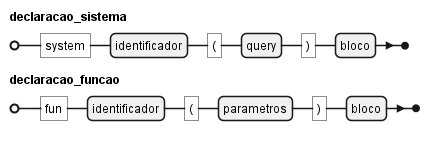
\includegraphics[width=0.45\textheight]{../diagrams/decl_sistema_funcao.png}
% 	\caption{Diagrama de sintaxe comparando declaração de sistemas e de funções.}
% 	\fonte{Elaboração própria com PlantUML feita com base no interpretador nosso e no de Jlox \cite{craftinginterpreters}.}
% 	\label{fig:decl_sistema_funcao}
% \end{figure}

% Vale ressaltar que semelhanças como essa estão presentes em outras partes da sintaxe da linguagem proposta, e foram intencionalmente feitas para facilitar a legibilidade e a facilidade de escrita através da familiaridade com outras linguagens, conforme discutido na \autoref{sec:design_linguagem}.

% Fora as semelhanças, as diferenças na implementação da linguagem proposta foram encontradas principalmente na semântica e na pragmática \cite{designconceptsinlanguages}, que foram adaptadas para suportar os conceitos de ECS.

% Ainda no exemplo de declaração de sistemas, a semântica foi feita de forma que o interpretador reconheça um sistema como uma função que atua sobre entidades e seus componentes de forma automática. Já a pragmática foi feita através da ligação da sua sintaxe com a API da biblioteca de ECS Flecs.

% A fim de melhor documentar o processo de desenvolvimento da implementação, a seção seguinte detalha as principais decisões feitas durante o desenvolvimento do interpretador.

% \section{Decisões de Desenvolvimento e seus Impactos}

% Esta seção tem a finalidade de documentar as principais decisões tomadas durante o desenvolvimento do interpretador em um só lugar, possivelmente servindo de referência para trabalhos futuros. Para cada decisão, será descrito o objetivo da decisão, a decisão em si, seu impacto no protótipo, e, caso aplicável, alternativas relevantes.

% \subsection{Escolha da Linguagem de Implementação}

% \begin{itemize}
% 	\item \textbf{Objetivo}: Escolher uma linguagem de programação adequada para implementar o interpretador, considerando fatores como suporte de bibliotecas, estruturas de dados expressivas e familiaridade do desenvolvedor;
% 	\item \textbf{Decisão}: A linguagem escolhida foi Rust, devido ao seu suporte a \textit{Algebraic Data Types} através de \texttt{enums} \cite{rustbook}, seu ecosistema com as bibliotecas necessárias, e a familiaridade do desenvolvedor com a linguagem;
% 	\item \textbf{Impacto}: A escolha de Rust tornou o processo de depuração extremamente previsível devido ao seu sistema de tipos rígido, além de permitir abstrações mais expressivas através de \texttt{enums} \cite{rustbook}.
% \end{itemize}

% \subsection{Escolhas de \textit{Design} da Linguagem}

% \begin{itemize}
% 	\item \textbf{Objetivo}: Integrar o ECS no \textit{design} da linguagem da forma mais simples e intuitiva possível, visto que o foco do trabalho está na implementação do interpretador;
% 	\item \textbf{Decisão}: O \textit{design} da linguagem foi feito adaptando a sintaxe de linguagens imperativas tradicionais para suportar os conceitos base de ECS: entidades, componentes e sistemas. Adicionalmente, a semântica e pragmática também seguem os conceitos de ECS.
% 	\item \textbf{Impacto}: Toda a sintaxe proposta pelo \textit{design} foi implementada e conseguiu servir de base para a semântica e pragmática necessárias para a integração com a biblioteca de ECS.
% 	% Como analisado na \autoref{tab:caracteristicas_nosso_design}, que compara \textit{design} da linguagem proposta com a biblioteca Flecs, nota-se que nosso \textit{design} marca todas as características relacionadas ao critério de legibilidade, porém não marca nenhuma característica relacionada aos critérios de facilidade de escrita e de confiabilidade.
% \end{itemize}

% \subsection{Representação das Abstrações Internas}

% \begin{itemize}
% 	\item \textbf{Objetivo}: Definir as estruturas de dados internas para representar as abstrações da linguagem proposta, como \textit{tokens}, expressões e instruções.
% 	\item \textbf{Decisão}: Utilizar \texttt{enums} do Rust para representar as abstrações internas, aproveitando o suporte a \textit{Algebraic Data Types} da linguagem \cite{rustbook}.
% 	\item \textbf{Alternativa}: Utilizar \texttt{structs} com campos para representar o tipo de cada abstração, como é feito em Jlox \cite{craftinginterpreters}. Essa alternativa foi descartada devido à superioridade dos \texttt{enums} quanto a código mais robusto.
% 	\item \textbf{Impacto}: A escolha de \texttt{enums} tornou o código mais robusto, já que em conjunto com \texttt{match}, o compilador do Rust consegue garantir que todos os casos possíveis de cada abstração sejam tratados \cite{rustbook}.
% \end{itemize}

% \subsection{Estratégia de Análise Léxica}

% \begin{itemize}
% 	\item \textbf{Objetivo}: Definir a estratégia de análise léxica para converter o código-fonte em uma sequência de \textit{tokens}. Idealmente, ela deve ser simples de implementar, já que o trabalho se trata de um protótipo.
% 	\item \textbf{Decisão}: A estratégia escolhida foi a implementação de um \textit{lexer} manual com \textit{iterators}, inspirado na implementação do Jlox \cite{craftinginterpreters}.
% 	\item \textbf{Alternativa}: Utilizar uma biblioteca geradora de \textit{lexers}. Inicialmente, a implementação do \textit{lexer} foi feita com a biblioteca Logos, porém, na época em que foi utilizada, não havia documentação suficiente sobre integração de erros customizados com a biblioteca, o que levou a decisão de implementar um \textit{lexer} manualmente.
% 	\item \textbf{Impacto}: A implementação do \textit{lexer} manual foi relativamente simples, com em torno de 180 linhas de código, e permitiu a implementação de erros customizados. Porém, caso a biblioteca Logos tivesse documentação suficiente na época, a implementação poderia ter sido mais simples e com menos linhas de código, como é possivel inferir dos exemplos na documentação da biblioteca \cite{logos}.
% \end{itemize}

% \subsection{Estratégia de Análise Sintática}

% \begin{itemize}
% 	\item \textbf{Objetivo}: Definir a estratégia de análise sintática para converter a sequência de \textit{tokens} em uma AST. Idealmente, ela deve ser simples de implementar, já que o trabalho se trata de um protótipo.
% 	\item \textbf{Decisão}: Diferente do \textit{lexer}, a implementação do \textit{parser} foi feita com uma biblioteca, Chumsky, que expõe uma API para criar \textit{parsers} de forma declarativa \cite{chumsky}.
% 	\item \textbf{Impacto}: A implementação do \textit{parser} com Chumsky foi relativamente simples, principalmente quando comparada com a implementação de \textit{parsers} manuais, como o do Jlox \cite{craftinginterpreters}. Devido a natureza declarativa da biblioteca, o código do \textit{parser} ficou extremamente parecido com as regras de produção da gramática, como comentado na \autoref{sec:analise_sintatica}. Isso facilitou a implementação e a depuração do \textit{parser}, que ficou com em torno de 120 linhas de código.
% \end{itemize}

% % TODO!
% % \subsection{Estratégia de Interpretação}

% % \begin{itemize}
% % 	\item \textbf{Objetivo}:
% % 	\item \textbf{Decisão}:
% % 	\item \textbf{Impacto}:
% % \end{itemize}

% \subsection{Escolha da Biblioteca de ECS}

% \begin{itemize}
% 	\item \textbf{Objetivo}: Escolher uma biblioteca de ECS adequada para integrar com o interpretador, considerando fatores como suporte da linguagem de implementação e documentação extensa;
% 	\item \textbf{Decisão}: A biblioteca escolhida foi Flecs, devido ao seu suporte a Rust através de \textit{bindings} e sua documentação extensa \cite{flecs}. Adicionalmente, o autor dessa biblioteca é o mesmo dos vários artigos sobre ECS usados neste trabalho. Além disso, Flecs é uma das poucas bibliotecas de ECS que suporta relacionamento entre entidades, o que será útil para as sugestões de trabalhos futuros \cite{flecs}.
% 	\item \textbf{Impacto}: A escolha da biblioteca Flecs facilitou sua integração com o interpretador, devido a sua documentação e artigos relacionados do autor. Porém, pelo fato de seu \textit{binding} para Rust não possuir declaração de componentes de forma dinâmica, a integração exigiu uma estratégia incomum, como descrita na \autoref{sec:interpretacao} \cite{flecs}.
% \end{itemize}

% % TODO!
% % \subsection{Representação Interna de Entidades, Componentes e Sistemas}

% % \begin{itemize}
% % 	\item \textbf{Objetivo}:
% % 	\item \textbf{Decisão}:
% % 	\item \textbf{Impacto}:
% % \end{itemize}

% \section{Viabilidade e Limitações da Solução}

% Por fim, esta seção serve como uma síntese dos resultados obtidos, avaliando a viabilidade e limitações da solução proposta e depois determinando se os objetivos do trabalho foram alcançados.

% Foi visto que o protótipo de interpretador conseguiu de fato interpretar programas na linguagem proposta, e que sua implementação se assemelha muito com a implementação de interpretadores tradicionais, salvo a fase de interpretação, que é onde há a ponte entre o interpretador e a biblioteca de ECS.

% A respeito de documentar as decisões de \textit{design} e implementação, a seção anterior o fez de forma detalhada, também incluindo os impactos de cada decisão no protótipo. De forma geral, as decisões tomadas durante o desenvolvimento do interpretador se mostraram acertadas, com impactos positivos na implementação.

% A respeito de limitações, a mais aparente é a falta de recursos que a linguagem proporciona, como controle de fluxo, funções, entre outros. Isso é intencional, visto que o trabalho propõe fornecer apenas um protótipo funcional, e não uma linguagem completa. Além disso, não houve nenhuma consideração quanto a desempenho, que é um dos principais benefícios do padrão ECS. Isso também foi intencional, de modo a reduzir o escopo do trabalho.

% Com o protótipo funcional, um registro das decisões tomadas durante o desenvolvimento, e a avaliação do trabalho como um todo e das decisões tomadas, conclui-se que os objetivos do trabalho foram alcançados.


\chapter{Conclusão} \label{ch:conclusao}

Este trabalho projetou e implementou de forma parcial um protótipo de interpretador para uma linguagem orientada ao padrão \textit{Entity Component System}, cumprindo a maioria dos objetivos inicialmente propostos, salvo a implementação completa da fase de interpretação.

O escopo incluiu a implementação das fases de análise léxica e sintática, além da formalização da fase de interpretação e do registro de escolhas de técnicas e bibliotecas utilizadas ao longo do desenvolvimento. Com o protótipo parcialmente funcional e a documentação de decisões tomadas completa, foi possível avaliar a viabilidade do trabalho, identificando tanto os pontos fortes quanto as limitações encontradas.

\section{Principais Resultados e Contribuições}

Como analisado no capítulo \ref{ch:analise_resultados}, o protótipo de interpretador conseguiu transformar o código fonte em uma AST completa, e identificado que sua implementação se assemelha muito com a implementação do interpretador Jlox, salvo a fase de interpretação, que é onde há a ponte entre o interpretador e a biblioteca de ECS.

A contribuição mais significativa deste trabalho é a implementação do protótipo de interpretador, que, atendendo a maioria dos objetivos propostos, serve como base para trabalhos futuros. Isso se deve pelo fato de que, assim como comentado na seção \ref{sec:justificativa}, a proposta deste trabalho não só é incomum, como também peca por não haver artigos e documentação sobre o assunto, tornando trabalhos futuros mais difíceis de serem feitos.

\section{Viabilidade e Limitações}

Assim como discutido na seção \ref{sec:viabilidade_limitacoes}, a implementação do protótipo de interpretador se mostrou viável quanto as fases de análise léxica e sintática. Porém, a implementação da fase de interpretação se mostrou inviável dentro do tempo disponível devido à dificuldade de representar tipos dinâmicos em
Rust e à falta de documentação sobre componentes dinâmicos na biblioteca de ECS escolhida.

Além disso, também na seção \ref{sec:viabilidade_limitacoes}, foi visto que o protótipo possui outras limitações, como a falta de recursos proporcionados pela linguagem e a ausência de considerações quanto a desempenho. Por mais que intencionais, essas limitações restringem o uso do protótipo a fins educacionais e de pesquisa, não sendo adequado para aplicações práticas.

\section{Sugestões para Trabalhos Futuros}

% TODO!
% Sabendo que o escopo deste trabalho foi propositalmente limitado, e que o objetivo era fornecer uma base para trabalhos futuros, há uma ênfase em sugestões para trabalhos futuros. A seguir, são listadas algumas sugestões, onde as três primeiras buscam resolver as limitações do protótipo, enquanto as duas últimas tomam liberdade criativa para sugerir novos recursos:

% \subsection{Explorar Otimizações e Analisar o Desempenho}

% \subsection{Dar Suporte a \textit{Queries} Mais Complexas}

% \subsection{Implementar um Agendador de Sistemas}

% \subsection{Explorar a Organização de Sistemas e Componentes}

% \subsection{Explorar o Conceito de Componentes e Sistemas como Entidades}

Sabendo que o escopo deste trabalho foi propositalmente limitado, e que o objetivo era fornecer uma base para trabalhos futuros, há uma ênfase em sugestões para trabalhos futuros. As sugestões mais relevantes são listadas a seguir:

\subsection{Devidamente Implementar a Fase de Interpretação}

A sugestão mais óbvia é implementar a fase de interpretação que não pôde ser integrada ao interpretador devido a restrições de tempo. Com isso, o protótipo se tornaria funcional por completo, permitindo que programas escritos na linguagem proposta sejam efetivamente interpretados.

\subsection{Explorar Otimizações e Analisar o Desempenho}

Explorar otimizações relacionadas a um interpretador orientado ao padrão ECS, também fazendo análises de desempenho. Isso se deve ao fato de que desempenho foi a motivação inicial por trás do ECS, e é muito provável que um interpretador como o deste trabalho possa se beneficiar de otimizações específicas relacionadas ao padrão.

Adicionalmente, muitos dos artigos autorados por Sander Mertens, autor muito citado neste trabalho, discutem otimizações relacionadas ao ECS, como a aplicação do \textit{design} orientado a dados ao ECS e a organização interna de entidades e componentes \cite{ecsfaq, ecsstorageinpics}. Esses artigos podem servir de base para trabalhos futuros que busquem explorar otimizações dentro do contexto deste trabalho.

\subsection{Dar Suporte a \textit{Queries} Mais Complexas}

O sistema de \textit{queries} implementado no protótipo é extremamente simples, suportando apenas a seleção de entidades que possuem todos os componentes listados. Sistemas de \textit{queries} mais complexos podem ser implementados na linguagem proposta, permitindo que o usuário seja mais expressivo ao definir quais entidades um sistema deve processar.

Baseado na documentação das bibliotecas de ECS Flecs e Bevy, será listado a seguir alguns exemplos de recursos que podem ser implementados em um sistema de \textit{queries} mais complexo:

\begin{itemize}
    \item \textbf{Exclusão de Componentes}: Permitir que o usuário especifique componentes que uma entidade não deve possuir para ser selecionada por um sistema \cite{flecs, bevy};
    \item \textbf{Componentes Opcionais}: Permitir que o usuário especifique componentes que uma entidade pode ou não possuir para ser selecionada por um sistema \cite{flecs, bevy};
    \item \textbf{Relacionamentos entre Entidades}: Permitir que o usuário especifique relacionamentos entre entidades para serem selecionadas por um sistema, já que atualmente, este conceito só é aplicado internamente pelo interpretador \cite{flecs, bevy};
    \item \textbf{Múltiplas Entidades em uma Única \textit{Query}}: Permitir que o usuário selecione componentes de múltiplas entidades em uma única \textit{query}, possibilitando que um sistema atue sobre os dados de mais de uma entidade por vez. Este tópico é discutido de forma aprofundada no artigo \textit{Why it is time to start thinking of games as databases} de \citeonline{ecsstorageinpics}.
\end{itemize}

\subsection{Explorar o Conceito de Componentes e Sistemas como Entidades}

Uma sugestão que talvez possa fazer a ideia de um interpretador orientado ao padrão ECS valer mais a pena é explorar como o conceito de componentes e sistemas tratados como entidades pode ser aplicado na linguagem proposta.

Com este conceito aplicado, seria possível atribuir metadados a componentes e sistemas, além de poder criar sistemas que operam sobre outros sistemas ou componentes, permitindo vários tipos de abstrações diferentes sem a necessidade de novas alterações na linguagem, caracterizando assim uma linguagem altamente ortogonal.

A seguir são listadas duas ideias de como esse conceito pode ser aplicado na linguagem proposta:

\begin{itemize}
    \item \textbf{Modificadores de Componentes}: Permitir que o usuário atribua metadados que alteram o comportamento de componentes\footnote{Este conceito já é utilizado na biblioteca Flecs, lá chamados de \textit{Traits} \cite{flecs}.}, como tornar um componente mutualmente exclusivo com outro;
    \item \textbf{Agendamento de Sistemas}: Permitir que o usuário defina a ordem de execução de um sistema logo ao lado de sua declaração, ou até mesmo criar sistemas que alteram a ordem de execução de outros sistemas.
\end{itemize}

Vale notar que, apesar dessas sugestões também poderem ser implementadas em uma biblioteca de ECS tradicional, uma linguagem pode torná-las mais acessíveis e expressivas através de sua sintaxe. O código \autoref{cod:exemplo_futuro} demonstra um exemplo de sintaxe que poderia ser usada para implementar essas duas ideias.

\codigoRust
\lstinputlisting[
    language=Rust,
    label=cod:exemplo_futuro,
    caption=Exemplo de sintaxe para implementar modificadores de componentes e agendamento de sistemas utilizando o conceito de componentes e sistemas como entidades.
]{../codes/exemplo_futuro.rs}
\vspace{-1em}
\fonte{Elaboração própria.}

No código \autoref{cod:exemplo_futuro}, nota-se a sintaxe que faz uso dos caracteres \texttt{@}, \texttt{(} e \texttt{)}. O caractere \texttt{@} indica uma inserção de componente em tempo de compilação, enquanto os caracteres \texttt{(} e \texttt{)} indicam um relacionamento entre entidades. Com ambos, é possível implementar tanto as ideias sugeridas quanto muitos outros conceitos que possam reutilizar a mesma sintaxe.

\section{Considerações Finais}

Com o protótipo funcional e documentado, foi possível alcançar os objetivos propostos, além de avaliar a viabilidade do trabalho e sugerir trabalhos futuros, tornando este trabalho uma base para pesquisas futuras na área de linguagens de programação orientadas ao padrão \textit{Entity Component System}.
